\documentclass[conference]{IEEEtran}
\IEEEoverridecommandlockouts
% The preceding line is only needed to identify funding in the first footnote. If that is unneeded, please comment it out.
\usepackage{cite}
\usepackage{amsmath,amssymb,amsfonts}
\usepackage{algorithmic}
\usepackage{graphicx}
\usepackage{textcomp}
\usepackage{xcolor}
\def\BibTeX{{\rm B\kern-.05em{\sc i\kern-.025em b}\kern-.08em
    T\kern-.1667em\lower.7ex\hbox{E}\kern-.125em X}}
\begin{document}

\title{Summer School Summary\

\thanks{Identify applicable funding agency here. If none, delete this.}
}

\author{\IEEEauthorblockN{wang yong}
\IEEEauthorblockA{\textit{ Central South University} \\
\textit{415 Lab }\\
Changsha, China \\
214712176@csu.edu.cn}
}

\maketitle

\begin{abstract}
This paper is about what I've learned in our summer school, there are four main parts, book reading, paper reading, experimental practice, and some basic skills learning like latex and git. During this time I get started to learn something about N D N(Named Data Networking), like how does it work, and how will it affect the structure of our networks in the future.
\end{abstract}

\begin{IEEEkeywords}
summer school, NDN,latex,git;
\end{IEEEkeywords}

\section{Introduction}
This paper is a brief summary of my learning contents and experiences in our summer school. The rest of the paper is organized as follows: Section II discusses some book reading. Section III introduces some related papers that are recommended by our seniors. In section IV, we do some experiments to get familiar with our test platform and have a better understanding of some mechanisms of Named Data Network. Section V discusses the basic common skills that we need to learn before we start our graduate years. Finally, section VI concludes the paper. 

\section{Book Reading}
In Summer school, I chose NDN (named data networking) as my research direction. I gradually set up some basic concepts of NDN. The main characteristics of NDN are embodied in the selection of diversified and flexible routing policies and the security mechanism based on data itself\cite{b1}. The most impressive points for me are NDN cache and forwarding mechanism.``Fig.~\ref{fig_fp}''and``Fig.~\ref{fig_fm}'' shows the NDN forwarding process and forwarding model, The details of how the router handles an interest packet are as follows:
\begin{itemize}
\item  First query CS according to Content Name. If the corresponding  Data package is found in CS according to the longest common prefix matching algorithm of Name, directly return the Data package to the interface receiving interest.
\item
If no matching data is found in CS, it is necessary to continue searching PIT according to name matching. If a matching item is found in PIT, add the interface in the Interest package to the interface list of the corresponding item in PIT. When a corresponding Data package is returned, distribute Data according to the interface column recorded in PIT, and store the Data package in CS.
\item
If (1) and (2) are not matched successfully, continue to search in FIB. If the corresponding item is found in FIB, it indicates that the node receives such an Interest packet for the first time, and the node knows which nodes to request data requested by such an Interest packet. In this case, the Interest packet is forwarded to other nodes according to the interface list of the corresponding prefix in FIB, and the Interest request needs to be added to PIT.
\item
 If there is no corresponding matching result in the above three structures, it indicates that the node cannot process the Interest packet, and this Interest packet needs to be discarded directly.
\end{itemize}

\begin{figure}[htbp]
\centerline{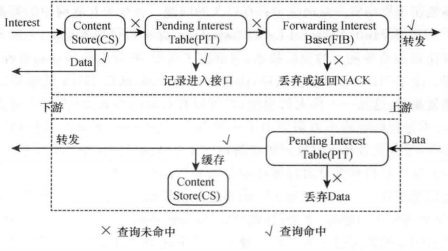
\includegraphics[scale=0.75]{fig_fp.png}}
\caption{NDN forwarding process.}
\label{fig_fp}
\end{figure}

\begin{figure}[htbp]
\centerline{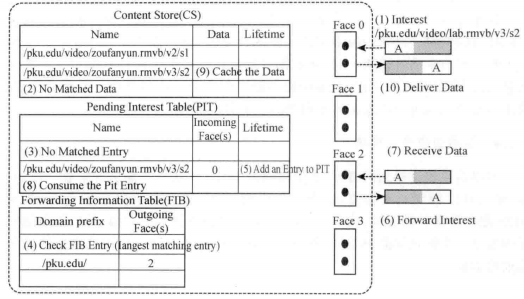
\includegraphics[scale=0.65]{fig_fm.png}}
\caption{NDN forwarding model.}
\label{fig_fm}
\end{figure}

\section{Paper Reading}
After learning some “textbook” knowledge, we studied basic papers and investigative papers and reported our understanding and confusion. Through reading these papers, I got some directions worth digging and research, and it also laid a foundation for my future research.

\subsection{Path Switching}\label{PS}
In \cite{b2}, it discusses fast-forwarding (mechanism for directing traffic to a specific path in a multipath or to a specific destination in a multidestination environment) by means of path tags.
``Fig.~\ref{fig_pl}'' shows how fast-forwarding is done (by skipping FIB table matching).
\begin{figure}[htbp]
\centerline{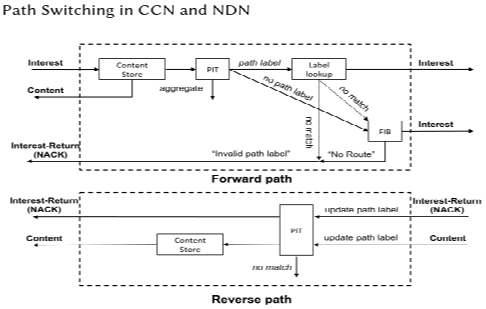
\includegraphics[scale=0.75]{fig_pl.png}}
\caption{Path Switching CCN/NDN forwarding plane.}
\label{fig_pl}
\end{figure}

\subsection{QoE-Aware Multi-Source Video Streaming}
Article \cite{b3} designs a QoE prediction model for ASDC that relies on scalable video streaming (SVC) based quality adaptive and representational delay effects. The ASDC algorithm considers the delivery of scalable video streams. When active switching occurs, it automatically adapts to each layer in the video stream based on the QoE model that describes the stall effect.

\subsection{NDN Live Video Broadcasting over Wireless LAN}
Paper \cite{b4} uses WiFi broadcast channel to deliver content from the access point to the user, leader-based mechanism to suppress the user's repeated requests, and receiver-driven rate control and loss recovery.
The ideas put forward in this paper aim at efficient and scalable real-time video streaming over wireless local area networks

\subsection{Scoped-Flooding for Content Discovery and Caching}
In the article  \cite{b5}, the scope flooding behavior is modeled with the theoretical model of network growth and utility. The influence of flooding on the topological structure of the information center network (ICN) is studied. Using the proposed loop model, we show that flooding can be confined to a small neighborhood to obtain most of the benefits from the region with a relatively low growth rate (i.e. the edge of the network). At the same time, two flood strategies (dynamic flood and static flood) are studied and their behaviors are compared.
\section{Experimental practice}
Experiment content: Modify NFD to observe the flow of NDN interest packets and data packets. First, I learned how to send and receive files and establish topology structure by NFDC instruction
Then I wrote a script  to establish  a static route structure between nodes
As shown in ``Fig.~\ref{fig_tp}''
Nodes a-e send interest packages prefixed with /test. Node g sends data packages prefixed with /test. When I printed the forwarding downstream entry of node f, I found that the data will be aggregated and distributed to A-E.

When I wrote this script, the main problem that needed to be solved is how to extract the specific content of the output information
(use grep and awk command combined to extract the required content). Also, this experiment impressed me a lot on how does a router sends and receives interest packets and data packages in NDN.
\begin{figure}[htbp]
\centerline{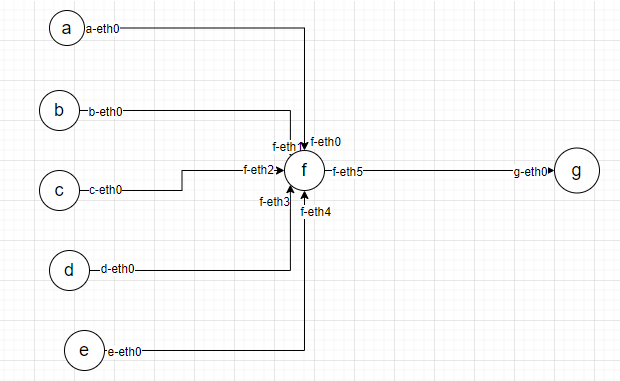
\includegraphics[scale=0.57]{fig_tp.png}}
\caption{ Test Topology.}
\label{fig_tp}
\end{figure}

\section{Basic skills learning}
\subsection{Git}
\begin{itemize}
    \item Basic uses. Git's basic uses range from initializing repositories, establishing connections to remote repositories, cloning remote repository content locally, adding it to staging, committing it to local repositories,  and pushing it to remote repositories
    \item
    Git merge. When some bugs appear in the project, you can create a new bug404 branch to fix the bugs and merge them into the main branch.
    The git-merge command can be used in two ways: in git-pull, to merge changes in another repository (i.e. Git pull = git fetch + git merge)
    Used for merging from one branch to another
    \item
    Conflict resolution. When different users push contents into the remote repository, conflicts may occur. In this situation, you can use the pull command to get the contents from the remote repository and merge them with the local repository. Take a text file as an example, the text file at this time will show the different modifications made by two users. At this time, remove the conflicts manually and upload again. After that, this conflict will be solved. 
\end{itemize}
\subsection{Latex}
\begin{itemize}
    \item Master some basic uses of latex include inserting words, formulas, pictures, tables, and references.
    \item Use overleaf to write latex documents online with Grammarly (an extension of Grammarly and Overleaf-Textarea)
    \item Use latexdiff to compare the differences between different versions and generates a new Tex file, visually showing the changes made between the two versions.
\end{itemize}

\section{Conclusion}
Through the study in summer school, I started some research on named data networking, gained some basic knowledge, understood some research directions worth digging in, and carried out some hands-on practice. At the same time, I also learned some common skills such as using Git and Latex, hoping to lay some foundation for my future research
\section*{Acknowledgment}
   This paper is my first attempt to learn latex, and there may be many mistakes.



\begin{thebibliography}{00}
\bibitem{b1} Lei Kai. Information Center Network and Named Data Network [M]. Peking University Press, 2015.
\bibitem{b2} Path switching in content centric and named data networks.  2017.
\bibitem{b3} [1] Sadat M N ,  Dai R ,  Kong L , et al. QoE-Aware Multi-Source Video Streaming in Content Centric Networks[J]. IEEE Transactions on Multimedia, 2019, 22(9):2321-2330.
\bibitem{b4} [1] Li M , Dan P , Zhang X , et al. NDN Live Video Broadcasting over Wireless LAN[C]// 2015 24th International Conference on Computer Communication and Networks (ICCCN). IEEE, 2015.
\bibitem{b5} [1] Wang L ,  Bayhan S ,  Ott J , et al. Understanding Scoped-Flooding for Content Discovery and Caching in Content Networks[J]. IEEE Journal on Selected Areas in Communications, 2018.
\end{thebibliography}


\end{document}
